

\section{Introduction} 

\subsection{Beamer 101}

% Frame
%--------------------------------------------------------------  

\begin{frame} 
	\frametitle{How to make an itemized list}

\begin{itemize} 

\item This is a beamer presentation template

\item It is customised with ISEG colors

\end{itemize}

\end{frame}

% Frame
%--------------------------------------------------------------  

\begin{frame} 
	\frametitle{How to make an itemized list}

You can also have text without bullets. And mix it with itemized lists in the same slide:

\begin{itemize} 

\item random item 1

\item random item 2

\end{itemize}

\end{frame}

% Frame
%--------------------------------------------------------------  

\begin{frame}
	\frametitle{itemized lists inside itemized lists}
	
\begin{itemize}

\item You can have itemized lists inside other itemized lists:

\begin{itemize}

\item This is a sub item
\item This is another sub item

\end{itemize}

\item You can even have sub sub items:

\begin{itemize}

\item subitem

\begin{itemize}

\item subsub item 1
\item subsub item 2
\item subsubitem 3

\end{itemize}

\end{itemize}

\end{itemize}

\end{frame}

% Frame
%--------------------------------------------------------------  

\subsection{Motivation}

\begin{frame}
	\frametitle{I built this template to}

\begin{itemize}

\item Help ISEG students

\item Improve my latex skills

\end{itemize}

\end{frame}

\section{Tables and mathematical expressions}


% Frame
%--------------------------------------------------------------  
\begin{frame}

\frametitle{Mathematical notation}

\begin{itemize}

\item \LaTeX is very useful to typeset mathematical notation. For example, this is the formula for Benford's law of first digits: $$ P(D_1=d_1) = \operatorname{log}\left(1+\frac{1}{d_1}\right), d_1\in \{ 1, \dots , 9\}$$

\item You can also use inline mathematical formulas instead. For example, this is a regression model: $y = \beta_0 + \beta_1 x_1 + \epsilon$.

\end{itemize}

\end{frame}

% Frame
%--------------------------------------------------------------  
\begin{frame}
	\frametitle{Mathematical notation}

This is the equation environment:

\begin{equation}
P(D_2=d_2) = \sum_{d_1=1}^{9} \operatorname{log} \left(1+\frac{1}{10\, d_1 + d_2} \right), d_2\in \{ 0, \dots , 9\}
\end{equation}

Note that with the equation environment equations are numbered.

\end{frame}

% Frame
%--------------------------------------------------------------  

\begin{frame}
	\frametitle{including pictures}

This picture is in the ``figures'' folder:

\begin{figure}
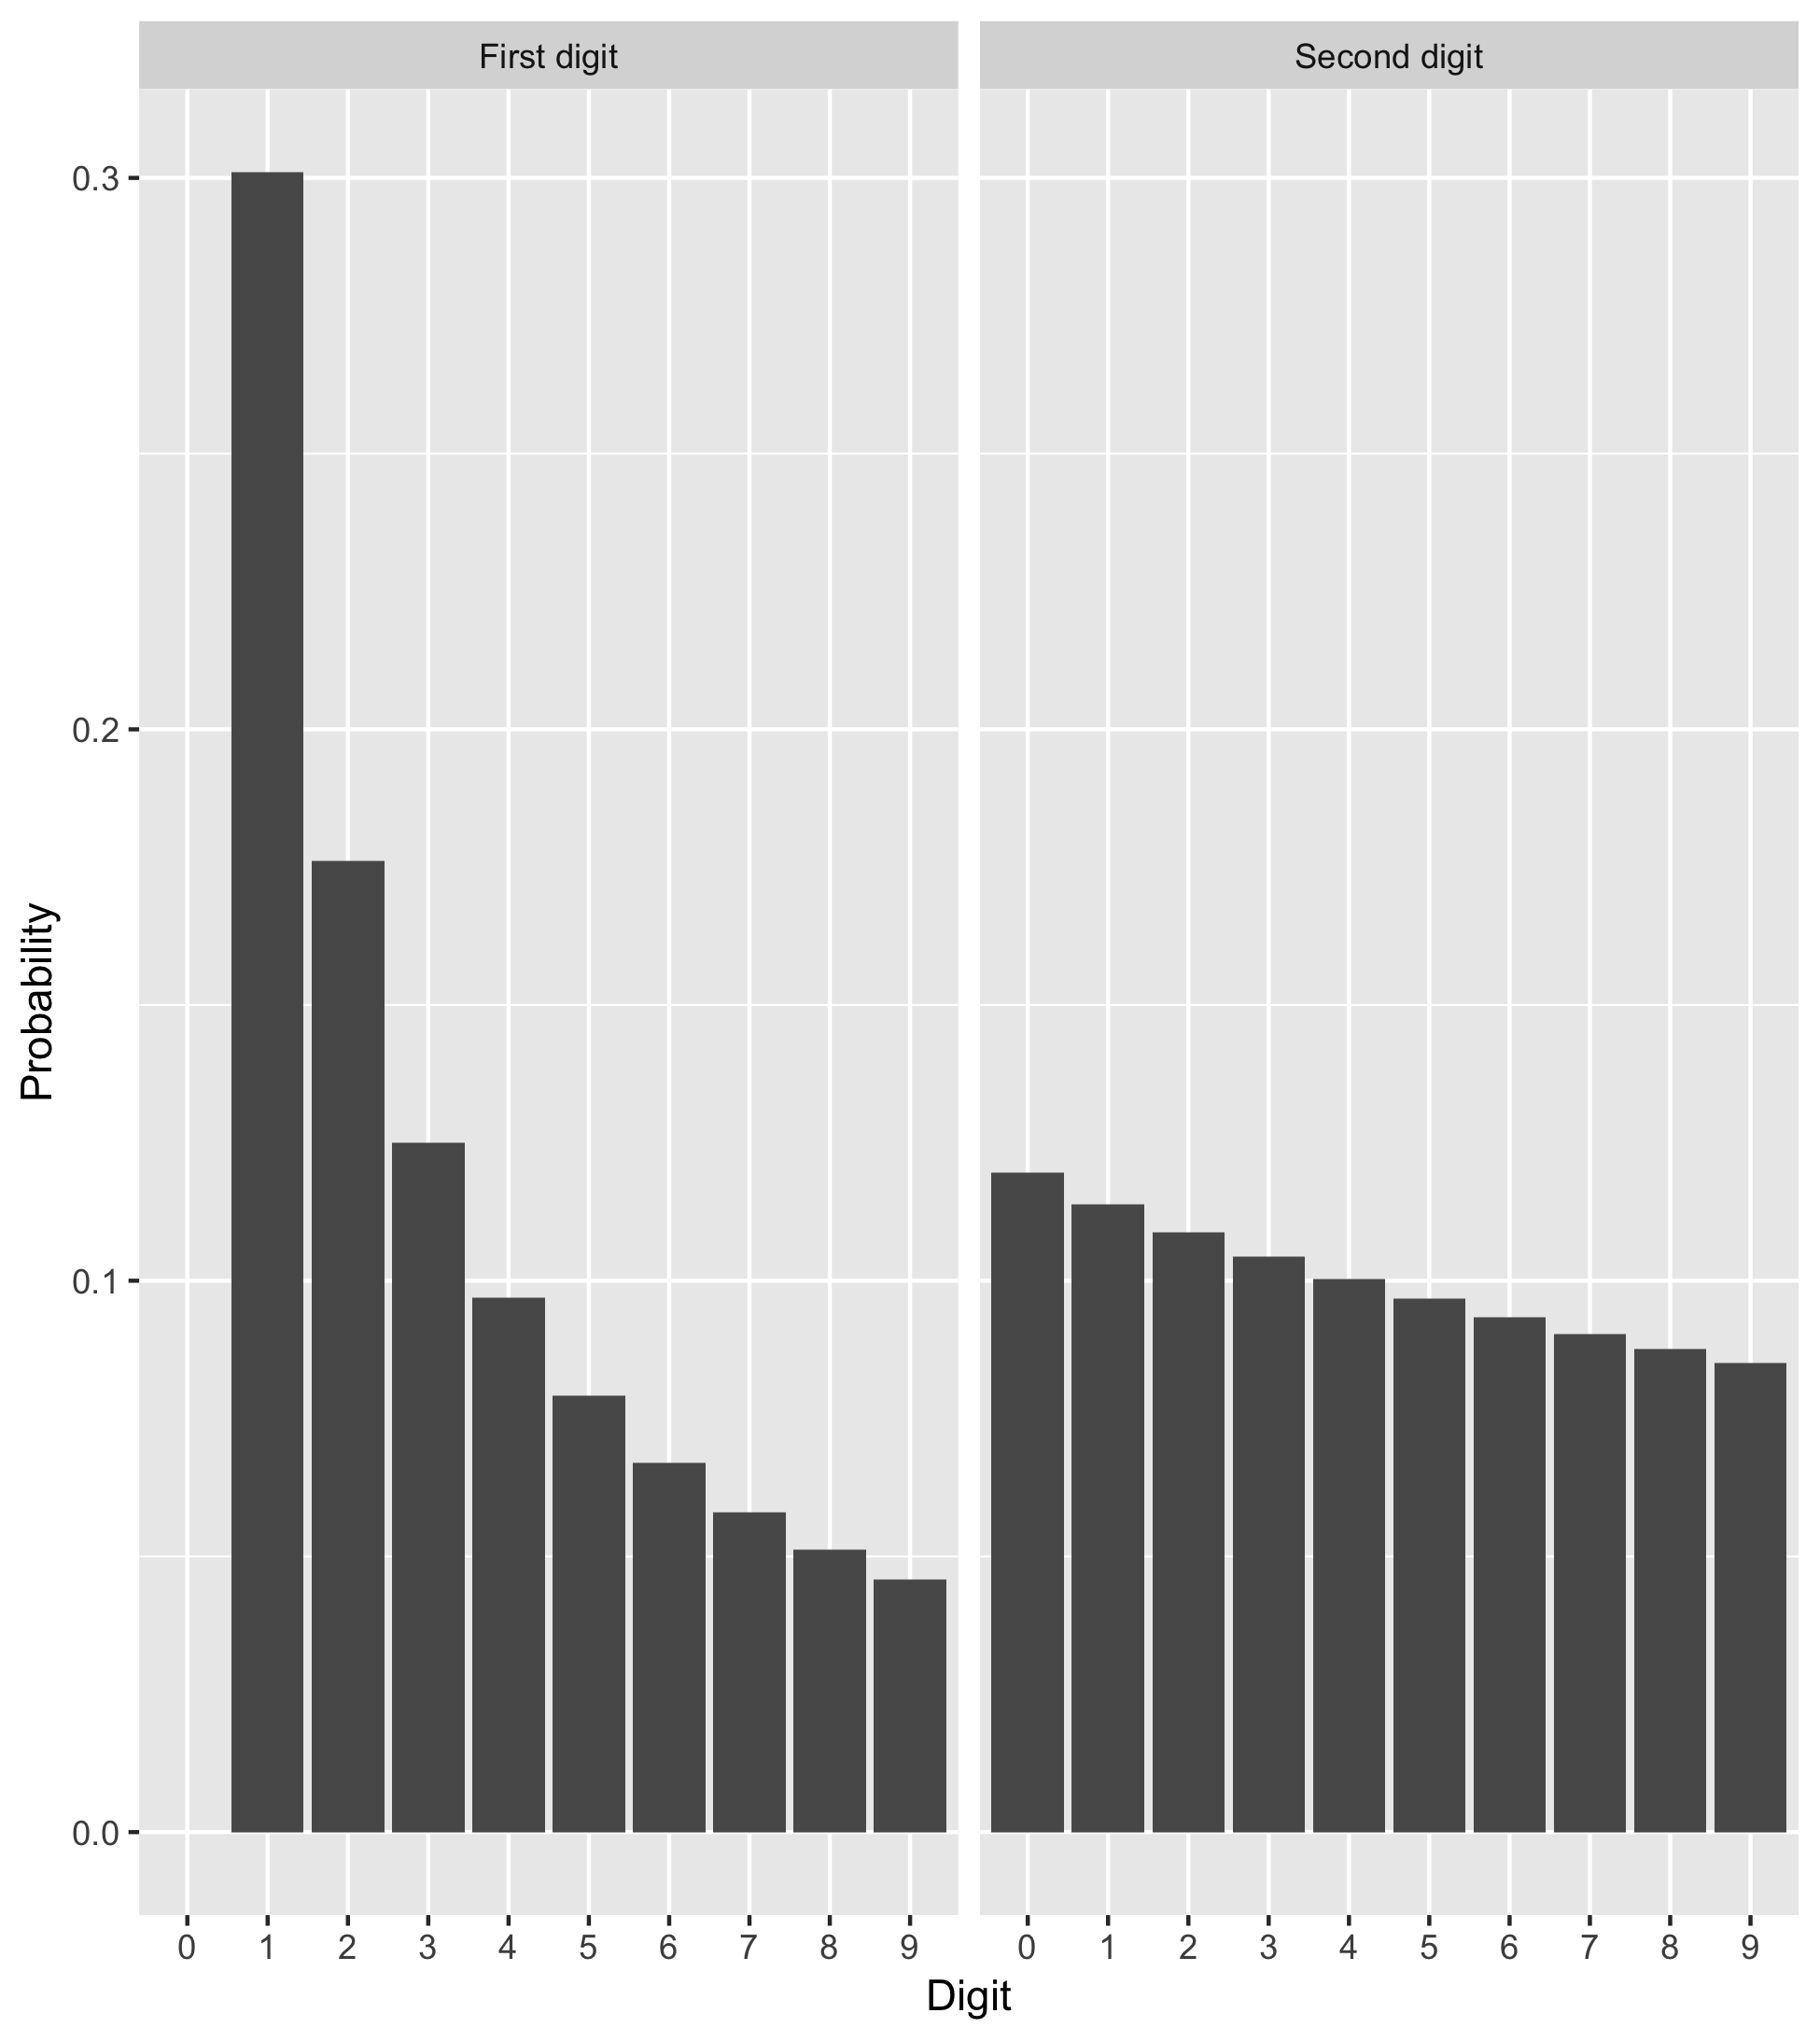
\includegraphics[scale=.075]{figures/benford.png}
\end{figure}

\end{frame}

% Frame
%--------------------------------------------------------------  




\subsection{Some complicated formulas}

\begin{frame}
\frametitle{Multinomial $\land$ Dirichlet Model}

\begin{itemize}

\item Bayesian model selection:

\begin{itemize}

\item Likelihood: $\bm{x}|\bm{\theta} \sim \mathcal{M}_k(N,\bm{\theta})$

\item Hypotheses:  $ H_0: \bm{\theta}=\bm{\theta_0} \,\,\,\, \text{vs} \,\,\,\,  H_1: \bm{\theta} \neq \bm{\theta_0}$

\item Prior: $\pi(\bm{\theta}|H_0)={1_{\bm{\theta_0}}(\bm{\theta_0})}$ and $\bm{\theta}|H_1, \bm{\alpha} \sim \operatorname{Dir}_k(\bm{\alpha})$ 

\item Marginal density: $m_i(\bm{x})=\int_{\Theta_i} f(\bm{x}|\bm{\theta})\pi(\bm{\theta}|H_i) \, d\bm{\theta} $, \, $i=0,1$

\begin{itemize}

\item  $m_0(\bm{x})=\frac{N!}{\prod_{i=1}^{k+1}x_i!}\prod_{i=1}^{k+1}{\theta_{0i}}^{x_i}$ 
\item  $m_1(\bm{x})= \frac{N!}{\prod_{i=1}^{k+1}x_i!}\frac{B(\bm{\alpha}+\bm{x})}{B(\bm{\alpha})}$ 

\end{itemize}

\item Bayes factor: $B_{01}(\bm{x}) = \frac{m_0(\bm{x})}{m_1(\bm{x})} = \frac{\prod_{i=1}^{k+1}{(\theta_{0i}}^{x_i}) \prod_{i=1}^{k+1}[\Gamma(\alpha_i)] \Gamma [\sum_{i=1}^{k+1}(\alpha_i+x_i)]}{\Gamma(\sum_{i=1}^{k+1} \alpha_i) \prod_{i=1}^{k+1}\Gamma(\alpha_i+x_i)}$

\end{itemize}	

\item Bayesian parameter estimation:

\begin{itemize}

\item Prior: $\bm{\theta}|\bm{\alpha} \sim \operatorname{Dir}_k(\bm{\alpha})$

\item Posterior: $\bm{\theta} | \bm{\alpha}, \bm{x} \sim \operatorname{Dir}_k(\bm{\alpha} + \bm{x}) \rightarrow$ Mean, mode, credible intervals.

\end{itemize}

\end{itemize}

\end{frame}

\begin{frame} 
	\frametitle{Binomial $\land$ Beta Model}

\begin{itemize}

\item Bayesian model selection:

\begin{itemize}

\item Likelihood: $x \sim \text{Bin}(N, \theta)$

\item  Hypotheses: $ H_0: {\theta}={\theta_0} \,\,\,\, \text{vs} \,\,\,\,  H_1: {\theta} \neq \theta_0$

\item Prior: $\pi(\theta|H_0)={1_{\theta_0}(\theta)}$ and $\theta| H_1 \sim \operatorname{Beta}($a$,$b$) $

\item Marginal density: $m_i(x)= \int_0^1 f(x|\theta)\pi(\theta|H_i)d \theta, \,  i=0, 1$

\begin{itemize}

\item $m_0(x)=\binom{N}{x} {\theta_0}^{x}{(1-\theta_0)}^{N-x}$ 

\item  $m_1(x) = \binom{N}{x}\frac{B(x+a, n-x+b)}{B(a,b)}$

\end{itemize}

\item Bayes factor: $B_{01}(x) = \frac{m_0(x)}{m_1(x)}  = \frac{\theta_0(1-\theta_0)^{N-x}\,\Gamma(a)\,\Gamma(b)\,\Gamma(n+a+b)}{\Gamma(a+b)\,\Gamma(n+a-x)\,\Gamma(x+a)}$ 

\end{itemize}

\item  Bayesian parameter estimation:

\begin{itemize}

\item Prior: $\theta \sim \operatorname{Beta}(a,b) $

\item Posterior: $\theta | x \sim \operatorname{Beta}(a+x, b+N-x ) \rightarrow$ Mean, mode, credible intervals

\end{itemize}

\end{itemize}

\end{frame}
